\documentclass[12pt]{article}

\usepackage{sbc-template}

\usepackage{graphicx,url}

\usepackage[brazil]{babel}   
%\usepackage[latin1]{inputenc}  
\usepackage[utf8]{inputenc}  
% UTF-8 encoding is recommended by ShareLaTex

     
\sloppy

\title{Padrões de Design de Serviços}

\author{João Marcos Ferreira\inst{1}, Kleonte Gomes\inst{2}, Rafael Tavares Rufino\inst{3} }


\address{Instituto Federal de Educação, Ciência e Tecnologia da Paraíba - Campus Cajazeiras (IFPB)\\
  Cajazeiras -- PB -- Brazil
  \email{joaomarccos.ads@gmail.com, kleonte email,
  rafaeltavares.rofino198@gmail.com}
}

\begin{document} 

\maketitle

\begin{abstract}
   resumo resumo resumo resumo resumo resumo resumo resumo resumo resumo resumo resumo resumo resumo resumo resumo resumo resumo resumo resumo resumo resumo resumo resumo resumo resumo resumo resumo resumo resumo resumo resumo resumo resumo resumo resumo resumo resumo resumo resumo resumo resumo resumo resumo resumo resumo resumo resumo resumo resumo 
\end{abstract}
   
\begin{resumo} 
  resumo resumo resumo resumo resumo resumo resumo resumo resumo resumo resumo resumo resumo resumo resumo resumo resumo resumo resumo resumo resumo resumo resumo resumo resumo resumo resumo resumo resumo resumo resumo resumo resumo resumo resumo resumo resumo resumo resumo resumo resumo resumo resumo resumo resumo resumo resumo resumo resumo resumo resumo resumo resumo resumo resumo
\end{resumo}


\section{O Que é SOA?}

Arquitetura orientada a serviços ou SOA (Service-Oriented Architecture) é descrita de forma diferente por vários autores, alguns o vêem como um estilo técnico de arquitetura que fornece os meios para integrar sistemas distintos e expor as funções de negócios reutilizáveis. Outros autores, no entanto, ter uma visão muito mais ampla:

SOA é uma abordagem arquitetural corporativa que permite a criação de serviços de negócio interoperáveis que podem facilmente ser reutilizados e compartilhados entre aplicações e empresas. [Gartner Group]


A arquitetura orientada a serviços é um estilo de design que orienta todos os aspectos da criação e utilização de serviços de negócios em todo o seu ciclo de vida (desde a concepção à aposentadoria). [Newcomer, Lomow, p. 13]


Arquitetura Orientada a Serviços (SOA) é um paradigma para organização e utilização de capacidades distribuídas que podem estar sob controle de diferentes domínios proprietários. [OASIS Ref Model]

De maneira simples, SOA é uma abordagem de negócios para criar sistemas de TI (Tecnologia de Informação) que permitem alavancar recursos existentes, criar novos recursos e, principalmente, estar preparado para inevitáveis alterações exigidas pelo mercado, obtendo mais produtividade e lucro para a empresa.


\section{Princípios de Design} 

Os Princípios de design são uma representação do paradigma de design orientado a serviços, eles estipulam boas praticas para construção de um sistema baseado em SOA bem implementado. A seguir estão os princípios de design de serviços listados por Thomas ERL(2009):

\begin{itemize}
\item Service Abstraction
\item Service Autonomy
\item Service Composability 
\item Service Discoverability
\item Service Loose Coupling
\item Service Reusability
\item Service Statelessness
\item Service-Orientation and Interoperability
\item Standardized Service Contract
\end{itemize}

Especificamente, a potencial relação entre princípios e padrões de projeto orientados a serviço pode ser resumido da seguinte forma:

    Princípios de design são aplicados coletivamente solução lógica, a fim de moldá-la de tal maneira que ela promove as principais características de design que suportam os objetivos estratégicos associados à computação orientada a serviços.
   Os padrões de design fornecem soluções para problemas comuns encontrados ao aplicar os princípios de design e ao estabelecer um ambiente adequado para a execução lógica concebida de acordo com os princípios de orientação a serviços.

\section{Padrões de Design}

No livro SOA Design Patterns de Thomas Erl, são apresentados diversos padrões, contudo serão descritos nesse artigo apenas os chamados padrões de serviços fundamentais, pois esses constituem um conjunto de padrões básicos de design que ajudam a estabelecer as características fundamentais do projeto de serviço através de uma sequência de aplicação sugerida. Coletivamente, esses padrões formam a aplicação mais básica de orientação a serviço.


\subsection{Agnostic Capability}

The subsection titles must be in boldface, 12pt, flush left.

\subsection{Agnostic Context}

The subsection titles must be in boldface, 12pt, flush left.

\subsection{Functional Decomposition}

The subsection titles must be in boldface, 12pt, flush left.

\subsection{Non-Agnostic Context}

The subsection titles must be in boldface, 12pt, flush left.

\subsection{Service Encapsulation}

The subsection titles must be in boldface, 12pt, flush left.


\section{Nessa seção fala das figuras e como vocês podem colocar elas no texto - Apagar depois}\label{sec:figs}


Figure and table captions should be centered if less than one line
(Figure~\ref{fig:exampleFig1}), otherwise justified and indented by 0.8cm on
both margins, as shown in Figure~\ref{fig:exampleFig2}. The caption font must
be Helvetica, 10 point, boldface, with 6 points of space before and after each
caption.

\begin{figure}[ht]
\centering
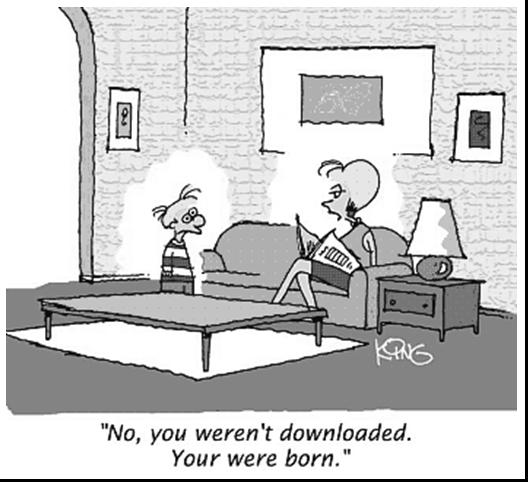
\includegraphics[width=.5\textwidth]{fig1.jpg}
\caption{A typical figure}
\label{fig:exampleFig1}
\end{figure}

\begin{figure}[ht]
\centering
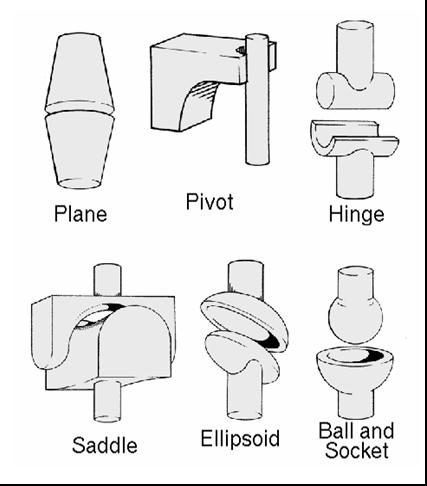
\includegraphics[width=.3\textwidth]{fig2.jpg}
\caption{This figure is an example of a figure caption taking more than one
  line and justified considering margins mentioned in Section~\ref{sec:figs}.}
\label{fig:exampleFig2}
\end{figure}

In tables, try to avoid the use of colored or shaded backgrounds, and avoid
thick, doubled, or unnecessary framing lines. When reporting empirical data,
do not use more decimal digits than warranted by their precision and
reproducibility. Table caption must be placed before the table (see Table 1)
and the font used must also be Helvetica, 10 point, boldface, with 6 points of
space before and after each caption.

\begin{table}[ht]
\centering
\caption{Variables to be considered on the evaluation of interaction
  techniques}
\label{tab:exTable1}
\smallskip
\begin{tabular}{|l|c|c|}
\hline
& Value 1 & Value 2\\[0.5ex]
\hline
&&\\[-2ex]
Case 1 & 1.0 $\pm$ 0.1 & 1.75$\times$10$^{-5}$ $\pm$ 5$\times$10$^{-7}$\\[0.5ex]
\hline
&&\\[-2ex]
Case 2 & 0.003(1) & 100.0\\[0.5ex]
\hline
\end{tabular}
\end{table}

\section{Considerações Finais}

All images and illustrations should be in black-and-white, or gray tones,
	excepting for the papers that will be electronically available (on CD-ROMs,
	internet, etc.). The image resolution on paper should be about 600 dpi for
	black-and-white images, and 150-300 dpi for grayscale images.  Do not include
	images with excessive resolution, as they may take hours to print, without any
	visible difference in the result. 
	
	\section{References}
	
	Bibliographic references must be unambiguous and uniform.  We recommend giving
	the author names references in brackets, e.g. \cite{knuth:84},
	\cite{boulic:91}, and \cite{smith:99}.
	
	The references must be listed using 12 point font size, with 6 points of space
	before each reference. The first line of each reference should not be
	indented, while the subsequent should be indented by 0.5 cm.
	

\bibliographystyle{sbc}
\bibliography{sbc-template}

\end{document}
